
\subsection{実験の目的,概要}
本実験では,0011および0010が入力されるたびに,1を出力する系列検出回路を設計する。
このとき,状態器械による順序回路記述で設計する。
作成した回路は,機能レベルシュミレーションと論理合成を行い,結果を確認する。

ICE計算機上の,ModelSim,Quartusを使用する。

この実験で,オートマトンの設計を回路にどう反映させるかの方法について,習得することを目的にする。

\subsection{実験方法}
\subsubsection{回路のHDL記述}
以下のような回路記述をm.v,テストベンチをtest\_m.vとして作成した。
\lstinputlisting[caption=m.v,label=m.v]{./src/m/m.v}
\lstinputlisting[caption=test\_m.v,label=testm.v]{./src/m/test_m.v}

\subsubsection{機能レベルシュミレーション}
作成したテストベンチをもとに,ModelSimで信号波形を出力した。
入出力の値が仕様通りの真理値表と一致することを確認した。

\subsubsection{論理合成}
以下の2ファイルを作成し,配置した。
\lstinputlisting[caption=m.qpf,label=m.qpf]{./src/m/m.qpf}
\lstinputlisting[caption=m.qsf,label=m.qsf]{./src/m/m.qsf}

作成した回路記述をQuartusでコンパイルし,論理合成とレイアウトを行った。
回路構成やロジックエレメント数,遅延時間について確認した。

\subsection{実験結果}
\subsubsection{機能レベルシュミレーション}
ModelSimで波形を作成した結果,以下のような波形になった。

\begin{figure}[H]
  \centering
  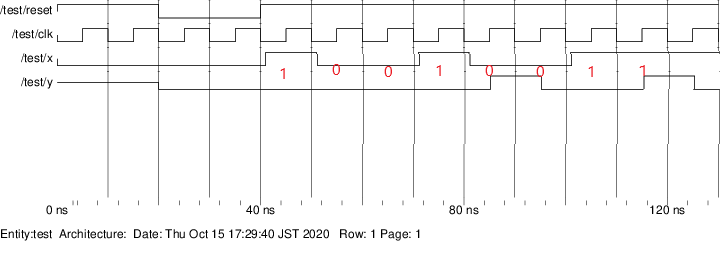
\includegraphics[width=\linewidth]{./src/m/mwave.png}
  \caption{mの波形}
\end{figure}

出力Yは,期待通り2回1を出力していた。

\subsubsection{論理合成}
論理合成の結果,以下のような回路が作られた。

\begin{figure}[H]
  \centering
  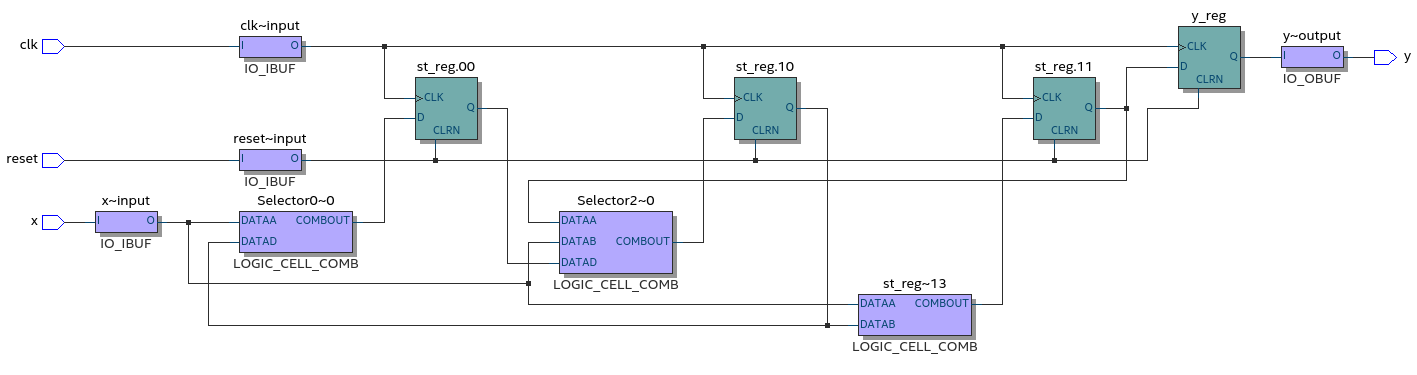
\includegraphics[width=\linewidth]{./src/m/mprint.png}
  \caption{mの回路}
  \label{mの回路}
\end{figure}

ロジックエレメント数は5だった。

回路全体の遅延時間は,以下のようになった。

\begin{figure}[H]
  \centering
  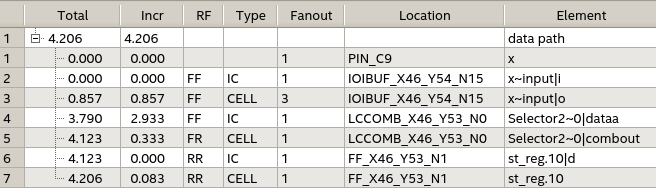
\includegraphics[width=\linewidth]{./src/m/mtiming.png}
  \caption{mの遅延時間}
\end{figure}

\subsection{考察}
\subsubsection{回路のHDL記述}
図\ref{設計したオートマトン}のような出力付きのオートマトンをもとにして,回路記述を行った。
レジスタに状態を記憶し,入力に応じて状態を遷移,出力する。

今回は,0010011のような系列に2回検出を行うオートマトンを設計した。

\begin{figure}[H]
  \centering
  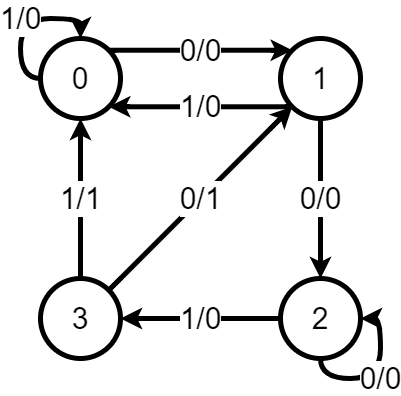
\includegraphics[width=5cm]{./src/m/mautomaton.png}
  \caption{設計したオートマトン}
  \label{設計したオートマトン}
\end{figure}

\subsubsection{機能レベルシュミレーション}
テストベンチでは,これまでの順序回路と同様な設定の後に,1→0→0→1→0→0→1→1という系列を10nsおきに入力している。
最初に0010が,次に0011が検出されることが期待されて,実際に2回検出されている。

\subsubsection{論理合成}
コード\ref{m.v}では,4状態のオートマトンと出力レジスタが宣言されているが,図\ref{mの回路}では,合成によって3つの状態と出力,論理演算のみで構成されていることがわかった。
状態として持っていた情報を,現在の状態と入力の演算として再定義することで,状態数を削減しているのだと予想する。\\

この実験で,オートマトンの設計を順序回路として記述する方法がわかった。
また,そのような回路は合成によって状態数が減ることがある,ということも確認できた。
